\subsubsection{WSO2 ESB}
\label{soa:tecnologias:wso2-esb}

WSO2 es una compañía de tecnología \eng{open source}, que proporciona \eng{middleware} de \gls{acro:soa}.  Es conocida por sus productos: \eng{Enterprise Service Bus}, \eng{API Management} y \eng{Governance} por nombrar algunos, utilizados por eBay, Boeing y Experian entre otros.

WSO2 fue fundada por el Dr. Sanjiva Weerawarana y Paul Fremantle en Agosto de 2005, y ha sido respaldada por Intel Capital, Toba Capital y Pacific Controls.  WSO2 ESB es rápido, ligero y versátil, 100\% \eng{open source}, está basado en los proyectos Apache Synapse\footnote{\url{http://synapse.apache.org}} y Apache Axis2\footnote{\url{http://axis.apache.org/axis2/java/core}}, y ha demostrado interoperabilidad con la mayoría de los \eng{stack} de Web Services, incluyendo Microsoft .NET WCF.

Utilizando WSO2 ESB se pueden implementar una gran variedad de patrones de integración empresarial (\eng{Enterprise Integration Patterns}, EIPs), incluyendo filtrado, transformaciones y ruteo SOAP, binario, XML y de mensajes de texto, atravesando los sistemas de la organización sobre HTTP, HTTPS, JMS, mail, entre otros.

\paragraph{Licencia}

WSO2 ESB se encuentra publicado bajo licencia Apache 2.0\footnote{La misma puede ser consultada en \url{http://www.apache.org/licenses/LICENSE-2.0}}.

\paragraph{Características principales}

\begin{itemize}
  \item Adaptadores a servicios en la nube: posee una tienda con más de 100 conectores\footnote{\url{https://store.wso2.com/store/assets/esbconnector}} como por ejemplo: CRM, ERP y redes sociales, entre otros.
  \item Soporte para diferentes tipos de transporte: HTTP, HTTPS, POP, IMAP, SMTP, JMS, AMQP, RabbitMQ, FIX, TCP, UDP, FTPS, SFTP, MLLP, SMS, MQTT y Apache Kafka.
  \item Formatos y protocolos: JSON, XML, SOAP 1.1, SOAP 1.2, WS-*, HTML, EDI, HL7, OAGIS, Hessian, Text, JPEG, MP4.
  \item Adaptadores para productos comerciales: SAP BAPI \& IDoc, IBM WebSphere MQ, Oracle AQ y MSMQ.
  \item Ruteo: basado en headers, basado en contenido, basado en reglas y basado en prioridades.
  \item Transformaciones: XSLT 1.0\/2.0, XPath, XQuery y Smooks.
  \item Alto rendimiento, alta disponibilidad, escalabilidad y estabilidad, soporta una cantidad de conexiones HTTP(S) concurrentes no bloqueantes en el orden de 1000 por servidor.
  \item Baja latencia en escenarios de alto rendimiento.
  \item Permite escalar horizontalmente.
  \item Estabilidad de ejecución a largo plazo con baja utilización de recursos.
  \item Permite balanceo de carga y failover para \eng{endpoints} de alta disponibilidad.
\end{itemize}


\paragraph{Instalación}

A continuación se detallan los pasos necesarios para la instalación y ejecución de WSO2 ESB, basándonos en su documentación oficial \footnote{\url{https://docs.wso2.com/display/ESB403/Installing+ESB+on+Linux+and+Solaris+from+Source+Distribution}}.  Previo a la instalación se debe verificar que se cumpla con los siguientes requisitos previos\footnote{\url{https://docs.wso2.com/display/ESB403/ESB+Installation+Prerequisites}}:

\begin{itemize}
  \item Java SE Development Kit (JDK)
  \item Apache ActiveMQ JMS Provider
  \item Apache Ant
  \item Apache Maven
\end{itemize}

Paso 1. Obtener el Pack de instalación.\\
Descargar la última versión de WSO2 ESB (para la descarga seguir las instrucciones \footnote{Las mismas pueden ser consultadas en \url{https://docs.wso2.com/display/ESB403/Obtaining+ESB}}).

\begin{listing}[H]
  \bashfile{src/03-capitulo-3/tecnologias/nodo-central/code/wso2/00-instalacion.sh}
  \caption{Comando para descargar los fuentes de WSO2 ESB}
  \label{soa:tecnologias:wso2:bash-descargar-fuentes}
\end{listing}

Paso 2. Extraer el archivo.\\
Una vez descargados los fuentes, extraer los archivos de instalación en el directorio \texttt{home}:

\begin{listing}[H]
  \bashfile{src/03-capitulo-3/tecnologias/nodo-central/code/wso2/01-instalacion.sh}
  \caption{Comando para descomprimir zip}
  \label{soa:tecnologias:wso2:bash-descomprimir-zip}
\end{listing}

Paso 3. Construir el WSO2 Enterprise Service Bus.\\
Ejecutar el siguiente comando para construir WSO2 ESB en el directorio de instalación:

\begin{listing}[H]
  \bashfile{src/03-capitulo-3/tecnologias/nodo-central/code/wso2/02-instalacion.sh}
  \caption{Comando para construir WSO2 ESB}
  \label{soa:tecnologias:wso2:bash-maven-clean}
\end{listing}

Paso 4. Configuración de la variable \verb|JAVA_HOME|.\\
Es necesaria la variable de entorno \verb|JAVA_HOME| para poder ejecutar WSO2 ESB.  La variable apunta al directorio donde se encuentra instalado \eng{Java Development Kit (JDK)}.

Editar el archivo \texttt{.bashrc} del directorio \texttt{home} y agregar la variable de entorno \verb|JAVA_HOME|.  Para configurar la variable \verb|JAVA_HOME|, seguir los siguientes pasos:

\begin{enumerate}
  \item Abrir el archivo \texttt{.bashrc} .
  \item Agregar las siguientes líneas al final del archivo: \\
        \begin{listing}[H]
          \bashfile{src/03-capitulo-3/tecnologias/nodo-central/code/wso2/03-instalacion.sh}
          \caption{Comandos para configurar variables de entorno}
          \label{soa:tecnologias:wso2:bash-configurar-variables-de-entorno}
        \end{listing}
  \item Guardar los cambios en el archivo. \\
  \item Para verficar la correcta configuración de la variable \verb|JAVA_HOME|, ejecutar el siguiente comando: \\
        \begin{listing}[H]
          \bashfile{src/03-capitulo-3/tecnologias/nodo-central/code/wso2/05-instalacion.sh}
          \caption{Verificamos la variable de entorno JAVA\_HOME}
          \label{soa:tecnologias:wso2:bash-verificar-variable-de-entorno}
        \end{listing}
\end{enumerate}

Paso 5. Acceder a la consola de administración del ESB.\\
El ESB ya se encuentra instalado, ahora procedemos a iniciar el servicio, para lo cual debemos realizar los siguientes pasos:

\begin{enumerate}
  \item Realizar una conección SSH al servidor.
  \item Ir al directorio \verb|<ESB_HOME>/bin|, donde \verb|<ESB_HOME>| es el directorio donde se encuentran los archivos de WSO2 ESB.
  \item Ejecutar el siguiente comando para iniciar el ESB:\\
        \begin{listing}[H]
          \bashfile{src/03-capitulo-3/tecnologias/nodo-central/code/wso2/06-instalacion.sh}
          \caption{Comando para iniciar el servicio WSO2 ESB}
          \label{soa:tecnologias:wso2:bash-inicio-de-servicio}
        \end{listing}
\end{enumerate}


\paragraph{Integración con nuestro diseño}

Para el nuevo diseño de la arquitectura, se implementaría WSO2 ESB como nodo central, en el cual se enrutarían todas las peticiones realizadas desde los diferentes clientes.  Detrás de WSO2 ESB tendríamos replicadas \textit{N} instancias de las \glspl{acro:api}, las cuales nos permitirían escalar horizontalmente de forma sencilla, dado que WSO2 ESB se encargaría de realizar el balanceo de la carga a cualquiera de estas instancias replicadas.  Delante del WSO2 ESB se instalaría WSO2 API Manager para administrar las \glspl{acro:api}, gestionar la autorización y el control de acceso a las mismas.

\begin{figure}[H]
  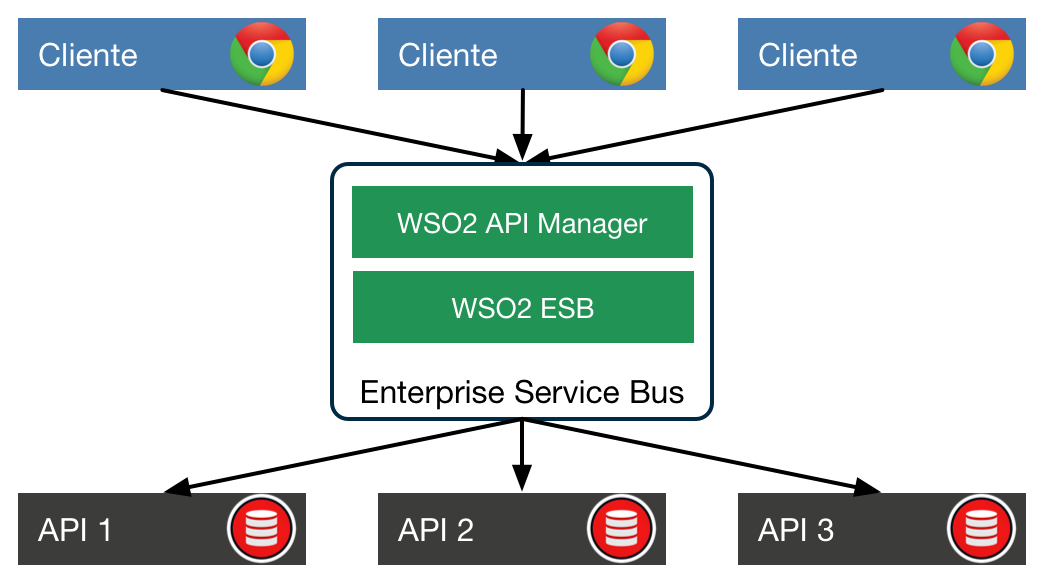
\includegraphics[width=\linewidth]{src/images/03-capitulo-3/tecnologias/wso2/wso2-esb-integracion-arquitectura.png}
  \caption{Esquema de integración de WSO2 ESB en nuestra propuesta}
  \label{fig:integracion-wso2-esb-arquitectura}
\end{figure}
